%%%%%%%%%%%%%%%%%%%%%%%%%%%%%%%%%%%%%%%%%%%%%%%%%%%%
% ITU Ph.D. Proposal Template
% Created by Farabi Ahmed TARHAN
% @2017 06 14
%%%%%%%%%%%%%%%%%%%%%%%%%%%%%%%%%%%%%%%%%%%%%%%%%%%%

\documentclass{ituphdreport}


\thesistitle{Multi Agent Planning Under uncertainty Using Deep Q Networks}
\writer{Farabi Ahmed}{TARHAN}
\studentid{511142108}
\department{Department of Aeronautical Engineering}
\programme{Aeronautical Engineering Programme}
\ddate{1st REPORT JANUARY 2018}
\tezyoneticisi{Assist. Prof. Dr. N. Kemal Üre}{Istanbul Technical University}
\juriBir{Prof. Dr. Gökhan İnalhan}{Istanbul Technical University}
\juriIki{Assist. Prof. Dr. Yıldıray Yıldız}{Bilkent University}

\begin{document}


\section{INTRODUCTION}

In this thesis progress report, the studies conducted at the first 6 month period of this study will be presented. As mentioned in the time plan of the thesis, it is aimed to develop a general framework that provides a basis for solving multiagent problems with deep q networks. In this context, a custom deep network framework and some benchmark problems designed and various q learning algorithms were tested over these benchmark problems. The outline of the progress report is as follows. In this section, an introduction is given and the scope of the thesis was reminded again. A time plan given in the approved proposal of the thesis was reintroduced in the 2nd Section. In Section 3, contribution of the studies conducted during the last six months within the whole thesis study is evaluated. The studies conducted during the last six months in accordance with the time plan are listed and their results are given in 4th Section. In Section 5, the studies included in time plan but not conducted are listed. In Section 6, the updated methodologies and their reasons are given. The next section explains the studies that is planned to be done for the next six months. In the last section, publications about the thesis is mentioned.

The proliferation of Unmanned Aerial Vehicles (UAVs) in the military and civil applications to substitute humans in dangerous or risky missions made UAVs very active research topic in many engineering fields. Control practices for a single vehicle or an agent had a major progress in executing advanced techniques such as adaptive control, intelligent control and robust control during the development of control theory. In the last decades, the idea of utilizing interconnected multiagent systems has gained more popularity in the continuation of the former developments, since lots of benefits can be obtained when complex solo systems are replaced by their heterogeneous and multiple counterparts \cite{rencao11}. Multiagent systems can be defined as a coordinated network of problem-solving agents, which cooperate to find answers to given problems that are otherwise impossible to accomplish or highly time-consuming jobs. In general, the required capabilities of collaborative scenarios are beyond the capabilities of a single agent \cite{glavic06}.

The most prominent reasons of why multiagent systems are advantageous when compared with solo systems can be given in terms of collaboration, robustness, and quickness in addition to scalability, flexibility and adaptivity \cite{clement04}. Since each member of a multiagent system executes small part of a complex problem, those given reasons occur inherently. Especially surveillance-like missions exploit multiple robots simultaneously since a team of robots obviously has a big return due to the geographic distribution over using just a single robot \cite{stone00}. While a single robot can execute the mission from just a single observation point, multiagent systems can perform the mission from lots of strategic points that are spread over a large area.

Due to its promising benefits, multiagent planning problems are becoming prevalent in engineering as an emerging sub-field of Artificial Intelligence (AI). Since the applications range across control of robotic missions, computer games, mobile technologies, manufacturing processes and resource allocation, it is also a widely acknowledged interdisciplinary engineering problem that draws the attention of researchers from distinct fields including computer science \cite{stone00}, aerospace engineering \cite{tomlin98}, operations research \cite{swaminathan98}, and electrical engineering \cite{glavic06}.

In this Ph.D. thesis, it is aimed to develop a highly scalable multiagent planning framework with the support of both centralized and decentralized setting for heterogeneous teams by using Deep-Q-Networks (DQN) technique to reduce dependency on the domain knowledge of the large-scale problems. Recent studies on machine learning and, in particular, on deep learning have demonstrated very promising successes in solving problems with complex and high-dimensional spaces \cite{silver2016mastering} \cite{zhang2016learning}\cite{mnih-dqn-2015}.

Centralized solutions, that require all the agents to communicate each other, will be developed using Multiagent Markov Decision Processes (MMDPs) as described in subsection \ref{sec:mmdp}. MMDPs are an extended version of standard MDP models to formulate multiagent decision-making problems. Most of the large-scale problems suffer from curse-of-dimensionality. Having high dimensional spaces such as multiagent planning problems impedes the convergence rate significantly. Centralized formulations also have large planning spaces since joint spaces of each agent is considered, hence these multiagent systems suffer from being exponential in the size of planning space as the number of agents increases \cite{redding2011approximate}. Therefore classical Dynamic Programming (DP) methods are not practical for such problems since they do not scale well. In order to reduce the computational complexity of the problem, approximate dynamic programming methods are developed to obtain at least near-optimal results. However, many of these algorithms depend on domain knowledge and extensive tuning. Recent advances in applying deep structures to multiagent systems show encouraging results \cite{hausknecht2015deep}\cite{tampuu2017multiagent}. By utilizing deep networks, the problems with large spaces can be solved by minor tuning that just comprises network topology. 

In real-world scenarios, the agents might not communicate each other always, due to communication limits. Having a limited or sometimes accessible communication makes some of the agents to be unaware of the states of other agents and the environment. In such scenarios, some precautions must be taken into account to let the team reach a common goal. In which situations, when agents are experiencing communication troubles, each agent should take care of themselves to keep the global reward of the mission acceptable at the same time. Hence, the technique that will be utilized should allow the agents, that receive separate observations, to take actions solely based on that local information \cite{amato13}. In this thesis Decentralized Partially Observable Markov Decision Processes (Dec-POMDPs) described in subsection ~\ref{sec:decpomdp} will be utilized to formulate multiagent decision making and control problem under uncertainty. A very recent study shows that Deep Q-Networks are a very promising method to deal with large-scale problems when studying decentralized systems \cite{chen2016decentralized}.

The scope of this thesis consists of developing a framework of both MMDPs and its decentralized counterpart Dec-MDPs. In order to evaluate the performance of the framework on UAV missions, a 3D Visual Software/Hardware-In-The-Loop UAV simulator will also be developed as described in subsection ~\ref{sec:simenv}. For the detailed evaluation of the decision-making system, 6 degree-of-freedom model of each member of the heterogeneous team, including an autonomous fixed-wing aircraft, an autonomous helicopter, and an autonomous multi-rotor, will be embedded in the simulation environment.

\section{TIME PLAN PRESENTED IN THESIS PROPOSAL}

As proposed in the proposal report, the envisioned time plan is depicted here again with shaded area in Figure \ref{fig:timeplan}. The shaded area shows the last six months that passed after the presentation of proposal report, and the items that had to be done so far. According to plan, the main work packages can be summarized as preliminary works, multiagent planning, decentralized multiagent planning, preparing simulation environment and thesis completion. In the preliminary phase as the main objective of this report, some elementary algorithms, such as value iteration, trajectory-based q-iteration, and deep-q-networks, were being implemented and tested in some benchmark environments especially grid-world and its derivatives. In second work package, multiagent planning algorithms will be developed and tested in the persistent surveillance environment. Afterward, the most challenging part of the thesis, decentralized multiagent planning, will be started to be developed. Followed by that work package, the 3D simulation environment will be developed to visualize the performance of the algorithms. In the last work packages, thesis writing will be started in parallel to writing journal drafts. As proposed in the proposal report, all of the thesis is still expected to be completed in 24 months.


\begin{figure}[h]
	\begin{center}
		\resizebox{6.3in}{!}{\includegraphics*{TimePlan2}}
	\end{center}
	\caption{Time plan presented in thesis proposal.
		\label{fig:timeplan}}
\end{figure}

%\input timeplan.tex


\section{CONTRIBUTION OF THE STUDIES CONDUCTED DURING THE LAST SIX  MONTHS WITHIN THE WHOLE THESIS STUDY}

In the last six months of the study, a custom deep network library and some benchmark problems, including grid-world, blocksworld, and rendezvous problems were developed. Various sets of value iteration methods were tested on these problems and their results were obtained. Besides these preliminary works, multiagent planning related studies are also started and some simulations were also conducted. Since these conducted works will serve a basis for the whole thesis study, it was really important to obtain such a general framework for both centralized and decentralized multiagent settings. 

\section{EXPLANATION OF THE STUDIES CONDUCTED DURING THE LAST SIX  MONTHS IN ACCORDANCE WITH THE TIME PLAN AND THEIR RESULTS} \label{sec:literature}
This section gives brief technical background on the methods that will be used in planning multiagent systems along with the introduction of MDPs and its extensions, dynamic programming, and deep neural networks. These preliminary tools will serve as a basis for the systems that are going to be developed throughout the thesis.

\subsection{Benchmark Problems} \label{sec:benchmarkproblems}
Benchmark problems are useful to evaluate the characteristics of algorithms with regard to their convergence rate, precision, performance, and robustness. These problems are generally designed as small-scale tasks that actually represents the real problem for which this study aims to find a generic solution. At this stage of the study, two different small-scale planning and decision making tasks such as blocks-world and grid world are generated and utilized to verify the developed various algorithms including, value iteration, trajectory-based value iteration, neural fitted q-iteration,  deep-q-networks, experienced replay and prioritized experience replay. The common theme between these problems is their dimensionality is increasing exponentially when the problem gets harder by increasing the blocks or agents. Before moving to real multiagent persistent surveillance problems, the developed algorithms need to prove their performance on these small-scale benchmark problems.


\subsubsection{Blocks World Planning Problem} \label{sec:blocksworldproblem}
Blocks world problem is selected since it is well defined, easily understood and sufficiently simple to evaluate the performances of various algorithms. Blocks world problem consists of an adequate set of identical blocks which are identified by numbers and includes the same number of slots on the floor. Each block can be placed either on the top of another block or on the slot. Figure \ref{fig:blocksworld} shows a random placement of blocks and goal states that belong to a blocks world planning problem that consists only 5 blocks. Since the stacking is assumed to be achieved by using a simple robot arm, only one block can be moved at a time. The robot arm can just move the blocks that are on the top of slots or stacks. There are only three types of actions, unstack, stack and do-nothing. The unstack operation requires only block number and removes the block from the top of the current stack to nearest free slot. The stack operation requires two parameters such as block number and slot number and places the block to the top of the indicated slot. 

\begin{figure}[h]
	\begin{center}
		\resizebox{5in}{!}{\includegraphics*{./images/blocksworld}}
	\end{center}
	\caption{Blocks world domain is a planning problem that consists a set of blocks and slots. 
		\label{fig:blocksworld}}
\end{figure}

In order to make the problem more realistic, an uncertainty is added. There is a small probability for the robot arm to drop the block while making an action. If dropping occurs, the block may fall either the left slot or the right slot. 

As seen in Figure \ref{fig:blocksworld_curseofdimensionality} since the number of states increases exponentially with the number of blocks, this planning problem suffers from the curse of dimensionality \cite{irodova2005reinforcement}. With just this impediment, this problem is really challenging as a single-agent planning problem.

\begin{figure}[h]
	\begin{center}
		\resizebox{3.5in}{!}{\includegraphics*{./images/blocksworld_curseofdimensionality}}
	\end{center}
	\caption{Blocks world domain suffers from curse of dimensionality. 
		\label{fig:blocksworld_curseofdimensionality}}
\end{figure}

\subsubsection{Grid World Planning Problem} \label{sec:gridworldproblem}
To illustrate simple single agent value iteration methods grid world planning problem can also be utilized. Grid world problem consists an agent, a partitioned area closed with walls, at least one goal point, and some non-compulsory blocked and penalty partitions. Our agent can move one step at a time and have 5 actions including do-nothing, up, down, left and right. In order to experience uncertainty, the outcome of each action is stochastic \cite{kochenderfer2015decision}. As seen in Figure \ref{fig:gridworld}, if the agent tries to go up, it will move to desired position with a probability of 0.8, but there is also a substantial chance to find itself in left or right grids. If the agent bumps itself to the outer walls or blocked grids, it will stay in the same position. While reaching to goal state has positive reward such as +1, reaching to the penalty states have negative reward such as -1.  Since there is a small but yet effective movement penalty such as -0.04, the main object of the problem is to reach the goal state with the smallest number of steps. The row and column position of the agent represents a state for the problem. The initial state can be selected either fixed or randomly depends on the requirements of the method that will generate a solution to the planning problem. 

\begin{figure}[h]
	\begin{center}
		\resizebox{5.75in}{!}{\includegraphics*{./images/gridworld}}
	\end{center}
	\caption{Grid world is one of the most used problem in reinforcement learning. 
		\label{fig:gridworld}}
\end{figure}

\subsubsection{Rendezvous Planning Problem} \label{sec:rendezvousproblem}
The rendezvous planning problem is derived from grid world problem. The configuration is same except the number of agents. This planning problem designed to evaluate the performance of algorithms that support multi-agent decision making. The main goal of this problem is to generate such a policy that allows the agents to meet at the point that has the biggest reward. 

\begin{figure}[h]
	\begin{center}
		\resizebox{3.5in}{!}{\includegraphics*{./images/rendezvous}}
	\end{center}
	\caption{Rendezvous planning problem is derived from grid world to evaluate multi-agent scenarios.
		\label{fig:rendezvous}}
\end{figure}

\subsection{Overview Of Planning Framework} \label{sec:overviewofplanningframework}
In order to implement algorithms and simulate infrastructure of physical systems, a unique and indigenous reinforcement learning framework is constructed. Since object-oriented programming practices typically use inheritance for code reuse and extensibility with the help of classes and prototypes, object-oriented architectures are applied when building infrastructure instead of other techniques such as procedural concepts. Since C++ programming language strongly supports the concept of object-oriented programming and reusability, the C++ classes are used in several modules. Besides C++, Python which is one of the most popular programming languages that supports object-oriented is also utilized on post-processing of simulations and 3rd-party tools.

\begin{figure}[h]
	\begin{center}
		\resizebox{5.75in}{!}{\includegraphics*{./images/inheritgraphcombined_1.jpg}}
	\end{center}
	\caption{Multilevel inheritance of multi-agent reinforcement learning framework.
		\label{fig:inheritgraphcombined_1}}
\end{figure}


As seen in Figure \ref{fig:inheritgraphcombined_1}, multilevel inheritance is used when deriving the classes. Multilevel inheritance allows the designer to use derive a class from another derived class. In order to provide a common and standardized interface that is appropriate for all the other external applications, the design is established onto abstract classes. By the help of abstract base classes, the derived classes can operate in a very similar way, while performing same functions with different implementations. In C++ abstract classes are implemented via virtual functions on the base classes. The base classes cannot be used to instantiate objects by their own and serve only as an interface. There are mainly 3 different abstract classes such as environment which models the physical environment of the problem, an agent which aims to solve the problem by collecting samples in a smart manner, and the representation which stores the quality values of previously experienced state-action pairs in the framework. Figure \ref{fig:inheritgraphcombined} depicts the UML class diagram generated by the Doxygen documentation tool of the framework in detail.
\begin{figure}
	\begin{center}
		\resizebox{6in}{!}{\includegraphics*{./images/inheritgraphcombined4.jpg}}
	\end{center}
	\caption{Class diagram of developed framework.
		\label{fig:inheritgraphcombined}}
\end{figure}

\subsection{Markov Decision Processes (MDPs)} \label{sec:mdp}
Many planning and decision making problems require choosing a sequence of decisions \cite{kochenderfer2015decision}. Markov Decision Processes (MDPs) are a common structure to analyze decision-making problems when outcomes are uncertain \cite{puterman2014markov}. The problems that are formulated by MDPs requires a known model and fully observable environment. MDPs, the sequential decision making formulations, is an extension of Markov Processes with added an action choosing mechanism. Markov Processes have the following properties:
\begin{itemize}
	\item Finite number of states and possible outcomes.
	\item The outcome at any state only depends on the outcome of the prior state.
	\item The probabilities are constant over time.
\end{itemize}

The MDP model consists states, actions, rewards, transition probabilities and discount factor. Hence, MDP is a tuple defined by,

\begin{equation}
\label{eq:mdptuple}
\mathcal {\langle  S, A, T, R,\gamma \rangle}, 
\end{equation}

where $S$ is the state space, $\mathcal A$ is the action space, $\mathcal{ T: S \times A \times S \rightarrow} [0,1]$ is the transition model, $\mathcal{R:S\rightarrow}\mathbb{R}$ is the reward model and $\gamma \in [0,1)$ is the discount factor. Discount factor balances current and future rewards and smoothly reduces the impact of rewards. It also enables to build a strategy to maximize overall reward at the expense of immediate rewards. $\mathcal{T}(s,a,s')$ is the transition probability of getting the state $s' \in \mathcal{S}$ by applying the action $a \in \mathcal{A}$ when in the state $s \in \mathcal{S}$. Let $s_k, a_k, r_k$ denote the state, the action and the reward at time step $k$. As MDP is a sequential control formulation, a trajectory can be denoted as $s_0, a_0, r_0, s_1, a_1, r_1, s_2, a_2, ...$, where the action $a_k \in \mathcal{A}$ is chosen according to a policy $\pi : \mathcal{S \rightarrow A}$ \cite{toksoz2012design}. The objective of the planning problem is to find a policy $\pi$ by maximizing the cumulative discounted reward for a given initial state $s_0$,

\begin{equation}
\label{eq:cumdiscreward}
Q^\pi (s,a) = \mathbb{E} \left[ \sum_{k=0}^{\infty}{\gamma^k r^k \vert s^0, a^0 = a, a^k = \pi(s^k)} \right],
\end{equation}

where $\mathbb{E}[.]$ is the expectation operator taken over the possible next states $s^{k+1}$, and $Q^\pi (s,a)$ is state-action value function under policy $\pi$. Obtaining the policy $\pi$ that maximizes the Eq. \ref{eq:cumdiscreward} will be provided in Section \ref{sec:planningwithmdps}. 


\subsection{Multiagent Markov Decision Processes (MMDPs)} \label{sec:mmdp}
Multiagent Markov Decision Processes (MMDPs) are extended version of MDPs to adapt it to multiagent problems which consists multiple agents trying to optimize an common objective. The MMDP formulation have lots of similarities with the exception that possible decisions, namely actions, are distributed among agents in the system \cite{boutilier1999sequential}.This formulations still requires each agent to observe the true state of the domain and coordinate on their taken actions \cite{amato13}. MMDP expands the above framework to a set of $n$ agents. A MMDP is also defined by a tuple,\begin{equation}
\label{eq:mmdptuple}
\langle n_a, \mathcal{S, A, T, R,\gamma \rangle}
\end{equation}
where $n_a\in \mathcal{Z}$ is number of agents and $\mathcal {\langle S, A, T, R,\gamma \rangle}$ is a MDP with factorized action space,
\begin{equation}
\label{eq:factorizedactions}
\mathcal{A} = \mathcal{A}_1 \times \mathcal{A}_2 \times \dots \mathcal{A}_{n_a},
\end{equation}
where $\mathcal{A}_i$ denotes the local action sets of agent, and $\mathcal{A}$ is the joint action set of the multiagent problem \cite{proper2009solving}. Note that the size of the action space is exponential in number of agents. In many multiagent problems, factorization of state space, transition models and rewards of the agents possible. By exploiting that structural property computationally efficient algorithms can be developed \cite{boutilier1999decision}. 

State space $\mathcal{S}$ is factorized into individual state spaces of each agent as follows,
\begin{equation}
\label{eq:factorizedstates}
\mathcal{S} = \mathcal{S}_1 \times \mathcal{S}_2 \times \dots \mathcal{S}_{n_a} 
\times \mathcal{S}^e_1 \times \mathcal{S}^e_2 \ldots \mathcal{S}^e_{n_e}
\end{equation}
where $\mathcal{S}_i$ denotes the individual states for $i^{th}$ agent, $\mathcal{S}^e_j$ is the state of external variable $j$, and $n_e$ is the dimension of the external states. Many real life problems such as multiagent traffic regulation problem, where the states of the traffic lights are associated to individual states, and position of the vehicles can be associated to external states, utilizes this assumption.

Transition dynamics can also be factorized as,
\begin{equation}
\label{eq:factorizedtransition}
\mathcal{T} = \mathcal{T}_1 \times \mathcal{T}_2 \times \dots \mathcal{T}_{n_a} 
\times \mathcal{T}^e_1 \times \mathcal{T}^e_2 \ldots \mathcal{T}^e_{n_e}
\end{equation}
where $\mathcal{T}_i : (\mathcal{S}_i \times \mathcal{S}^e) \times \mathcal{A}_i \times \mathcal{S}_i \rightarrow [0,1]$,
$i=1,\dots ,n_a,$ 
and $\mathcal{T}^e_i :
\mathcal{S} \times \mathcal{A} \times \mathcal{S} \rightarrow [0,1]$, 
$i=1,\dots,n_e$. Note that, while transition dynamics of each agent only depend on the agents external states, individual states and individual actions, external transition dynamics depend on joint action space, and joint space. Hence the dynamics of the external states are not decoupled from agents, they are influenced by actions of all agents.

The reward can also be decomposed as,
\begin{equation}
\label{eq:factorizedreward}
\mathcal{R} = \mathcal{R}_1 + \mathcal{R}_2 + \dots + \mathcal{R}_{n_a}
\end{equation}
where each $\mathcal{R}_i : \mathcal{S}_i \times \mathcal{S}^e \times \mathcal{A}_i \rightarrow \mathcal{R}$. Each local reward is individually dependent on the local states, local actions and joint space of external states.

Since MMDP is basically an MDP that has a specific structure that can be factorized, modeling multiagent problems become easier. Thus MMDP problems can be solved as an MDP using algorithms described in Sec. \ref{sec:planningwithmdps}. However, since even factorized MMDPs have large state and action spaces that are exponential to the number of agents, those classical approaches usually does not scale well for multiagent problems.

\subsection{Planning with MDPs} \label{sec:planningwithmdps}
The goal of solving an MDP is to find the optimal policy $\pi^*$ that maximizes state-action dependent value function $Q^\pi(s,a)$ defined in Eq. \ref{eq:cumdiscreward} as,
\begin{equation}
\label{eq:cumdiscreward}
Q^\pi (s,a) = \mathbb{E} \left[ \sum_{k=0}^{\infty}{\gamma^k r^k \vert s^0, a^0 = a, a^k = \pi(s^k)} \right],
\end{equation}
It can be showed that $Q^\pi (s,a)$ satisfies the Bellman Equation \cite{bellman1958dynamic}.
\begin{equation}
\label{eq:bellmanQ}
Q^\pi (s,a) = \mathbb{E}_{s'} \left[ 
\mathcal{R}(s,a,s') + \gamma Q^\pi (s',\pi(s')
\right]
\end{equation}
In particular, the optimal policy $\pi^*$ is defined as,
\begin{equation}
\label{eq:optimalpolicy}
\pi^*(s) = \argmax_{a\in \mathcal{A}} Q^{\pi}(s,a)
\end{equation}
where, for a given state, the action with the biggest value in the value function is chosen through all other action candidates. 

\subsection{Dynamic Programming }
In the Artificial Intelligence community, the problems formulated with MDPs utilize dynamic programming techniques \cite{sutton1984temporal}.
The main idea of using those formulations is to find an accurate decision criterion for each state. Dynamic programming is a method of simplifying a complex decision problem by breaking it into a collection of simple decision problems, solving each of those simple ones and storing their values. Dynamic programming algorithms can be classified as value iteration, policy iteration and policy search \cite{busoni:1}. In this work value iteration algorithm will be used to find the optimal decision.

In contrast to deterministic systems, there are also some transition probabilities that depend on current state and action. The system will evolve through those probabilities. Since the new state is determined by especially the decisions given in that state, the available decisions that can be applicable should be ranked \cite{bertsekas:1}. This is where the value functions come into play. By the help of value functions, the system can easily decide an action over another for each state.

The classic value iteration algorithm updates state-action/decision values by sweeping through all state and action space and applying Bellman Update, until update error decreased to applicable level \cite{bertsekas:1}. The expectation of Eq. \ref{eq:bellmanQ} can be expanded over transition probability as follows;
\begin{equation}
\label{eq:bellmanQ}
Q(s,a) = \sum_{s'\in \mathcal{S}} \mathcal{T}(s,a,s') [\mathcal{R}(s,a,s') + \gamma max_{a'} Q (s',a')]
\end{equation}

State-action dependent value iteration algorithm can be given as,

\begin{algorithm}[H]
	\begin{algorithmic}
		\Statex \textbf{Input:} $MDP, \eta $
		\Statex \textbf{Output:} $Q^*$
		\Procedure{ValueIteration}{$\mathcal{X}$, $A$, $g$, $f$, $\alpha$}
		\State $Q(s,a) \leftarrow $ initialize arbitrarily  \textbf{for} $s\in \mathcal{S}, a\in \mathcal{A}$
		\Repeat \ at every iteration $l = 0,1,2,...$
		\For{every $(s,a)$}
		\State $Q_{l+1} \leftarrow \sum_{s'\in \mathcal{S}} \mathcal{T}(s,a,s') [\mathcal{R}(s,a,s') + \gamma max_{a'} Q_l (s',a')]$
		\EndFor
		\Until{$(Q_{l+1}-Q_l) < \eta$} \\
		\Return $Q^* = Q_l$
		\EndProcedure
	\end{algorithmic}
	\caption{Q-Value Iteration}
	\label{alg:value-iteration}
\end{algorithm}

Figure \ref{fig:tabularsingleagent} shows a simulation result for a single agent grid world. A 3x4 small grid world problem is simulated with 0.8 discount factor. Q-Value iteration and tabular representation are utilized. As seen from the plot that, the agent can reach approximately maximum reward in a very small amount of iterations.

\begin{figure}[h]
	\begin{center}
		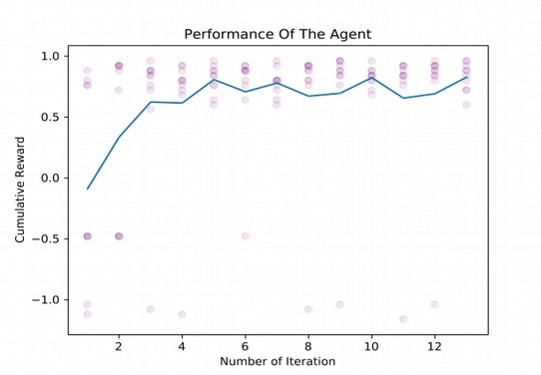
\includegraphics[width=0.6\textwidth]{tabularsingleagent}
	\end{center}
	\caption{Single agent grid world simulation with tabular q-value iteration.
		\label{fig:tabularsingleagent}}
\end{figure}

\subsection{Trajectory Based Value Iteration }
Since dynamic programming works on the complete model, standard value iteration algorithm requires scanning the entire state-action space. As sweeping the whole planning space leads to much higher time complexity, for large planning problems value iteration is intractable \cite{zhou2015trajectory}. To overcome this problem, an extension of the value iteration method named as trajectory based value iteration (TBVI) is utilized \cite{geramifard:1} as shown in Algorithm \ref{alg:tbvi}. This algorithm has some differences when compared with value iteration. Besides its efficient planning space sweeping, it works with any linear function approximator including neural networks. The samples are gathered using the e-greedy policy which is an exploration and exploitation dilemma that collects trajectories in the form of $(s_0, a_0, r_0, s_1, a_1, ...)$. The algorithm automatically terminates when the update error in a consequent set of trajectories is below a predefined threshold.

\begin{algorithm}[H]
\begin{algorithmic}
	\Statex \textbf{Input:} $MDP, \alpha, L_1 $
	\Statex \textbf{Output:} $\pi$
	\Procedure{TBVI}{$\mathcal{S}$, $A$, $\epsilon$, $\alpha$}
	\State $Q(s,a) \leftarrow $ initialize arbitrarily  \textbf{for} $s\in 
	\mathcal{S}, a\in \mathcal{A}$
	\While{time left}
	\For{$(s,a)$ in a trajectory following $\pi^\epsilon$}
	\State Create $L_1$ samples: $s'_j \sim \mathcal{P}^a_{s.}, j=1,...,L_1$
	\State $Q^+(s,a) \leftarrow \frac{1}{L_1} \sum_{j=1}^{L_1} \mathcal{R}^a_{ss'_j} + \gamma max_{a'} Q (s'_j,a')$
	\State $\delta \leftarrow Q^+(s,a) - Q(s,a)$
	\State $\bf{\theta} \leftarrow \theta + \alpha\delta\phi(s,a)$
	
	\EndFor
	\EndWhile
	\Return $\pi$ greedy with respect to $Q$
	\EndProcedure
\end{algorithmic}
\caption{Trajectory Based Value Iteration}
\label{alg:tbvi}
\end{algorithm}

Figure \ref{fig:trajectorysingleagent} shows the simulation result for the same setting that is given in previous subsection. Trajectory based value iteration can also reach the optimum reward but it takes more iterations to converge. 

\begin{figure}[h]
	\begin{center}
		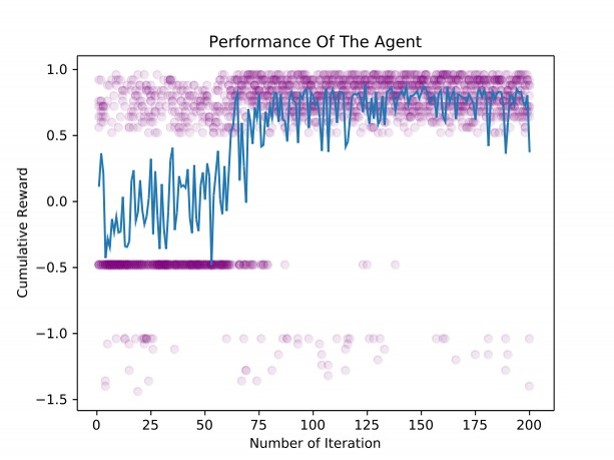
\includegraphics[width=0.6\textwidth]{trajectorysingleagent}
	\end{center}
	\caption{Single agent grid world simulation with tabular trajectory based q-value iteration.
		\label{fig:trajectorysingleagent}}
\end{figure}

\subsection{Representations}
The way of storing the values for state and action pairs is called representation. Representation is separated into two main groups as tabular representations and compact representations \cite{geramifard:1}. In tabular representation, each state and action pair is stored in a look-up table. This way of representation gives optimal decisions. However, due to the curse-of-dimensionality for large state-action spaces, this type of representation requires huge memory in practical applications. Because of that drawbacks pushed the researchers to move away from tabular representations to more compact representations. In compact representations, the value of each state-action pair is estimated implicitly using given features. One possibility is to use a multilayer perceptrons as called as neural networks to overcome drawbacks of former technique.

\subsection{Deep Network}
The deep network is a technique inspired from how human brain works to make possible the machines to learn from data. In contrast to customary neural network applications, in the reinforcement learning context, there is no readily available training set to train the algorithm. Each training label should be inferred during iterative value updates. In Figure~\ref{fig:networkstructure} a neural network structure is depicted.

\begin{figure}[h]
	\begin{center}
		\resizebox{6in}{!}{\includegraphics*{./images/networkstructure.png}}
	\end{center}
	\caption{An example of network structure for 4x3 Gridworld with single hidden layer.
		\label{fig:networkstructure}}
\end{figure}

The network is modeled by the output function $y(\textbf{x},\textbf{w})$ where $\textbf{x}$ is vector of inputs and $\textbf{w}$ is vector of weights. The output function $y$ varies with changes in the weights. Our goal is to find the weight vector that minimizes the error. The error is due to the improper values of weights results from a difference between the desired output and the network output for that training data pair. That pair includes an input vector $\textbf{x}$ and a label vector $\textbf{y}$. Define a topology;

\begin{equation}
\begin{aligned}
T=\{L_1, L_2, ..., L_m \}
\end{aligned}
\end{equation}

where $m$ is the number of total layers and $ L_i $  is the $ i^{th} $  layer of the network.

\subsection{Training with Backpropagation}
Training of a network can be done by following steps;

1. Given a training set:

\begin{equation}
\begin{aligned}
D = \{(x^{(1)} ,y^{(1)}) ... (x^{(t)} ,y^{(t)})\}
\end{aligned}
\end{equation}

where $t$ is the total number of training pair.

2. For each element of training set, feed-forward the input $x^{(d)}$ and obtain output $y^{(d)}$, then calculate error:

\begin{equation}
\begin{aligned}
E^{(d)}(\boldsymbol{w}) = \frac{1}{2} \sum_{i=1}^{|L_m|} (y^{(d)}_i - o^{(d)}_i)^2
\end{aligned}
\end{equation}

where $d$ stands for $d^{th}$ training data and ${|L_m|} $ stands for number of neurons in the $m^{th}$ layer.

3. Then calculate the gradient:
\begin{equation}
\begin{aligned}
\nabla E^{(d)}(\boldsymbol{w})=\left [
\frac{\partial E^{(d)}}{\partial w^1_{11}},
\frac{\partial E^{(d)}}{\partial w^1_{12}},
...,
\frac{\partial E^{(d)}}{\partial w^m_{ij}}
\right]
\end{aligned}
\end{equation}

4. Update the weight using gradient descent:

\begin{equation}
\begin{aligned}
\Delta \boldsymbol{w} &= -\eta \nabla E(\boldsymbol{w}) \\
\boldsymbol{w} &= \boldsymbol{w} + \Delta \boldsymbol{w}\\
w_i &= w_i - \eta \frac{\partial E}{\partial w_i},
\end{aligned}
\end{equation}

\subsection{Batch Training}
Processing the data to train the deep learning algorithms can be done various ways. The most naive way that comes to mind at first is to train the network using each data sequentially without skipping anyone. If the computation is applied on all of the data, it is called as online data processing. When the size of training data is large,  it probably needs a substantial amount of time to complete iterations and converge to the optimum. In order to use the resources effectively including time and computational power, the training can be done over some portion of data as seen in Figure \ref{fig:batchdata}. Thıs portion is called as batch size and the process is called as batch data processing in the neural networks lingo. Using batch data when training the algorithm has some more advantages including higher stability and the ability to be processed by parallel computing units. 
\begin{figure}[h]
	\begin{center}
		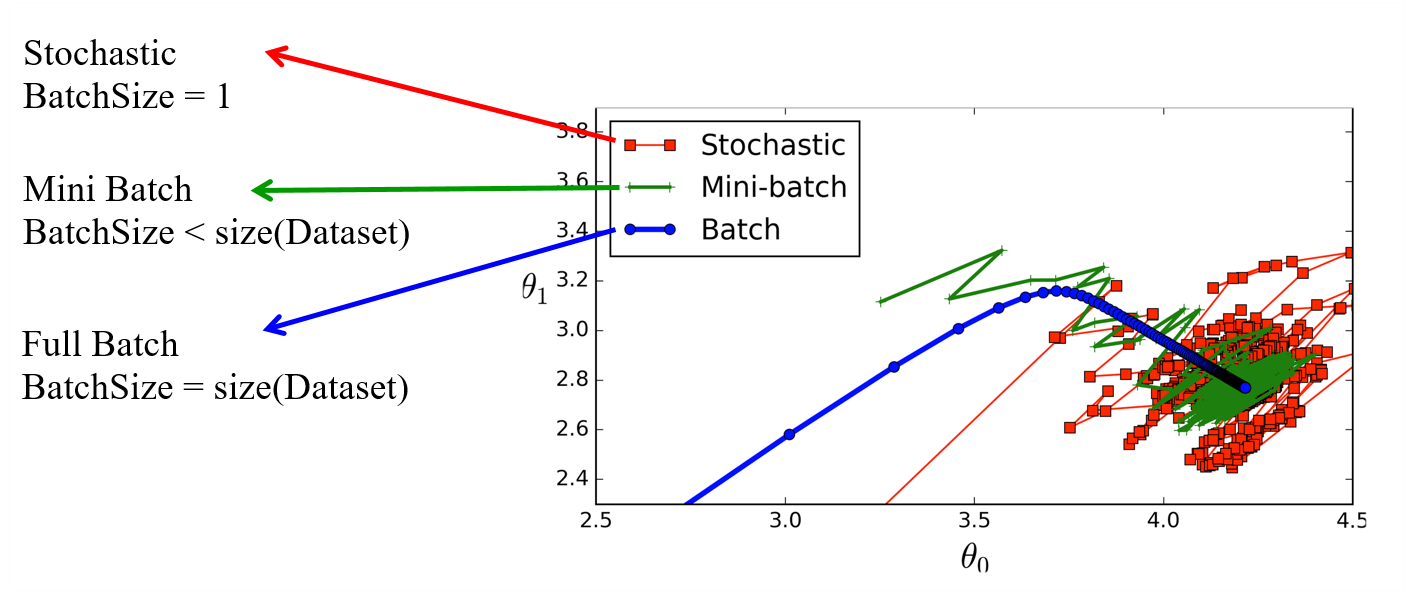
\includegraphics[width=0.85\textwidth]{batchdata}
	\end{center}
	\caption{Stochastic and batch optimization.
		\label{fig:batchdata}}
\end{figure}

Batch data processing has some more parameters that need to be tuned. Batch size is the number of training examples in only one forward/backward pass of a network. The higher the batch size the more memory space the system will need. The training examples are stored in a data structure called as a first-in-first-out memory block. The memory size specifies the length of this data structure. If the memory reaches the maximum amount of elements, the new coming training examples remove the older elements from the memory. The epoch number defines the number of a forward and a backward pass of the batch while learning. As seen in comparison table given in Figure \ref{fig:batchcomparison} the setting in the green row stabilized the multiagent grid world problem faster than the others. 

\begin{figure}[h]
	\begin{center}
		\resizebox{3in}{!}{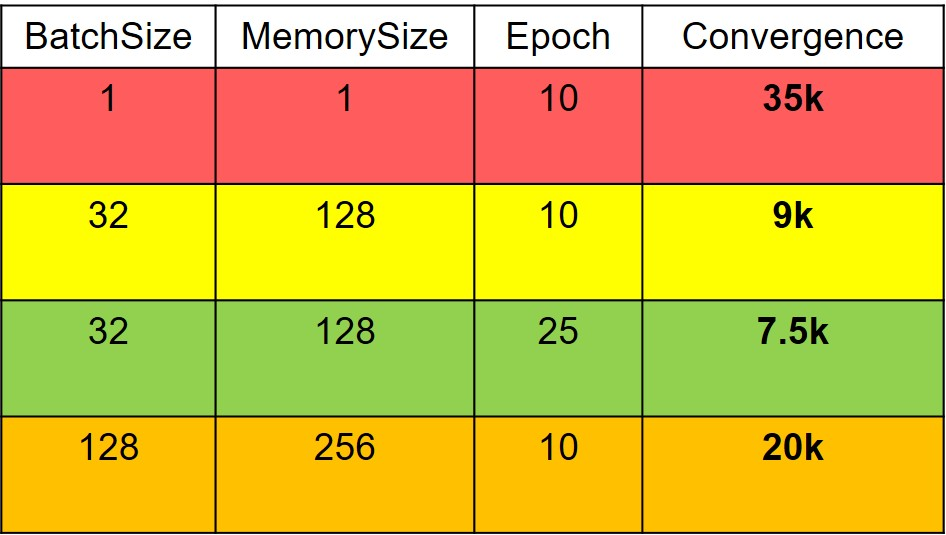
\includegraphics[width=1\textwidth]{batchcomparison}}
	\end{center}
	\caption{Batch learning comparison with different hyperparameters.
		\label{fig:batchcomparison}}
\end{figure}

\subsection{Experience Replay}
The fully connected network used in Deep-Q-Networks tends to forget the previous experiences as new samples collected. As the importance of batch data processing mentioned before, the experience replay technique addresses the issue of how the elements should be selected from memory into the batch list \cite{mnih-dqn-2015}.  To perform experience replay we store the agent's experiences as $e_t = (s_t,a_t,r_t,s_{t+1})$ in a memory buffer. These experience elements consist of state, action, reward, and next state. The populated memory is used to select the elements of the batch using uniform distribution. Then the batch list is replayed when training network. This randomized mechanism allows the learning algorithm to be more stable by removing the correlations in the observation sequence. It also brings together a more smooth convergence over the changes in the experienced data distribution.


\subsection{Deep-Q-Networks Structure} \label{sec:TODO!PAR}
In this study, it is aimed to develop a highly scalable multiagent planning framework with the support of both centralized and decentralized setting for heterogeneous teams by using Deep-Q-Networks (DQN) technique to reduce dependency on the domain knowledge of
the large-scale problems. Recent studies on machine learning and, in particular, on deep learning have demonstrated very promising successes in solving problems with complex and highdimensional spaces \cite{mnih-dqn-2015}. In both centralized and decentralized setting, there are two main solution methods such as exact
and approximate approaches. Exact approaches such as dynamic programming (DP) guarantees
optimal solutions but suffers from computational and memory requirements due to scalability
issues. Since exact solution methods have some major limitations, approximate approaches are
needed to improve the scalability of large-space multiagent problems. In order to mitigate these
limitations, an approximated novel approach known as Deep-Q-Networks (DQN) will be used
to represent non-linear functions. Deep neural networks are exceptionally good at coming up with good features for highly structured data. DQN could represent the Q-function with a neural network, that takes the state as input and outputs the corresponding Q-value for each action. With the help of Experince Replay DQN's successfully approximate the q values. Figure \ref{fig:deepmultiagent} and \ref{fig:deepmultiagent2} shows multiagent simulation results in a 5x5 Grid World environment. As it can be seen in the second plot that, an multiagent problem can be solved with DQN with only $ \%15 $ parameters of the tabular representation.

\begin{figure}[h]
	\begin{center}
		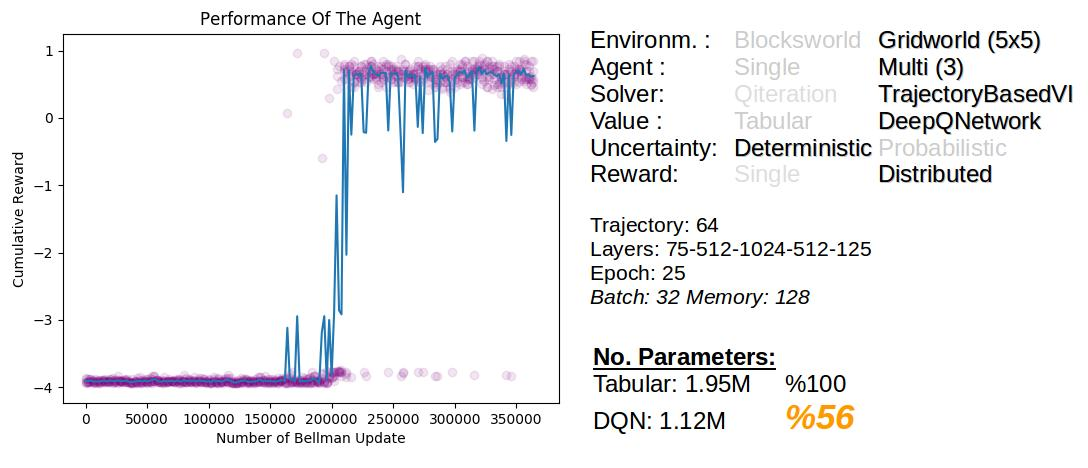
\includegraphics[width=1\textwidth]{deepmultiagent}
	\end{center}
	\caption{Multiagent simulation with deep network.
		\label{fig:deepmultiagent}}
\end{figure}
\begin{figure}[h]
	\begin{center}
		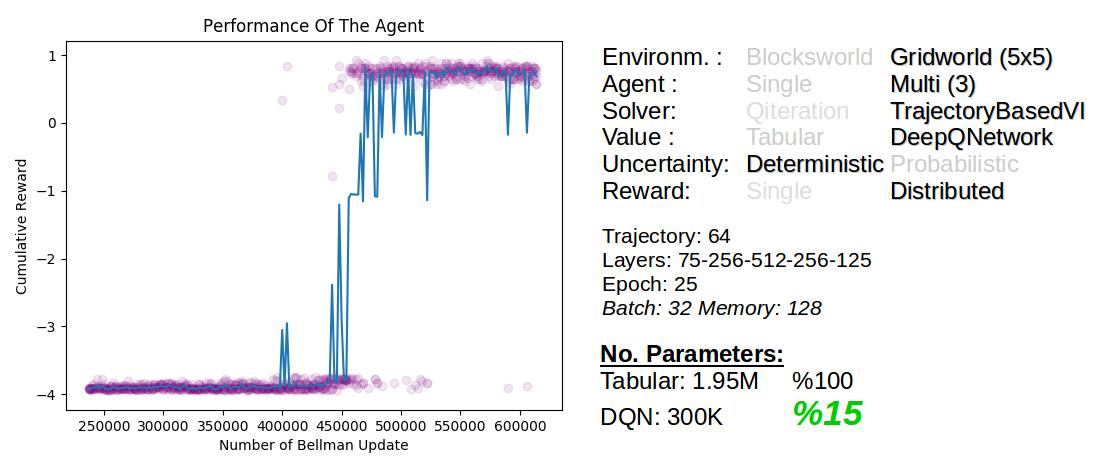
\includegraphics[width=1\textwidth]{deepmultiagent2}
	\end{center}
	\caption{Multiagent simulation with smaller network.
		\label{fig:deepmultiagent2}}
\end{figure}

\subsection{Prioritized Experience Replay}
Prioritized experience replay is an extension of replay memory mentioned above, that addresses also which experiences should be replayed to making the most effective use of experience storage for learning \cite{schaul2015prioritized}. Since most of the problems included in Reinforcement Learning exhibit sparse rewards, reaching these rare rewards and making inferences about the problem requires different novel techniques. Coping with sparse rewards is one of the biggest challenges in Reinforcement Learning \cite{andrychowicz2017hindsight}. One can classify the state transitions as 'surprising' when an agent happens upon a positive reward and 'boring' when an agent gets nothing different as the outcome of an action \cite{kaelbling1996reinforcement}. Therefore some transitions have importance over the others. In order to be able to learn faster, the learning algorithm should focus on the experiences that are more important using the prioritized experience learning. 

In order to differentiate the surprising and boring transitions, PER uses the temporal difference (TD) error that simply computes the difference between target network prediction and q-network prediction to assign a priority over the received experiences. A big TD error results in a higher priority. 

\begin{equation}
\begin{aligned}
TD_{error} = | Q(s,a) - Q^*(s,a)|
\end{aligned}
\end{equation}

This TD error can be transformed into a priority:

\begin{equation}
\begin{aligned}
p_i = [TD_{error}(i) - \epsilon]^\alpha
\end{aligned}
\end{equation}

where $i$ is the index of experience, $p_i$ represents the proportional priority of experience $i$, $\epsilon$ is a small positive constant that prevents transitions not being revisited once theirerror is zero. The exponent  $\alpha$ determines how much prioritization is
used, with $\alpha$ = 0 corresponding to the uniformly selected experience as in Experience Replay. Figure \ref{fig:prioritizeder2} demonstrates how the system behaves for different alpha values. Then the $p_i$ priority can be translated to a probability, so one can simply sample it from the replay memory using its probability distribution. An experience $i$ has the following probability of being picked from the replay memory:

\begin{equation}
\begin{aligned}
P_i = \frac{p_i}{\sum{k}{}p_k}
\end{aligned}
\end{equation}

\begin{figure}[h]
	\begin{center}
		\resizebox{3in}{!}{\includegraphics*{sumtree}}
	\end{center}
	\caption{Sum-Tree data structure is utilized by prioritized experience replay.
		\label{fig:sumtree}}
\end{figure}


When a problem requires large data sets and memory buffers, searching from memory for the element that has the highest priority can be intractable in practice with usual data structures.  However,  as shown in Figure \ref{fig:sumtree} if Sum-Tree data structure is used, the searching can be completed at $O(logN)$ complexity. In sum-tree, the value of a parent node is the sum of its children. Only leaf nodes store the transition priorities and the internal nodes store the sums of their own child. To sample a minibatch of size $k$, the range $[0, p_total]$ is divided into $k$ ranges \cite{schaul2015prioritized}. Then a value is uniformly sampled from each range.

\begin{figure}[h]
	\begin{center}
		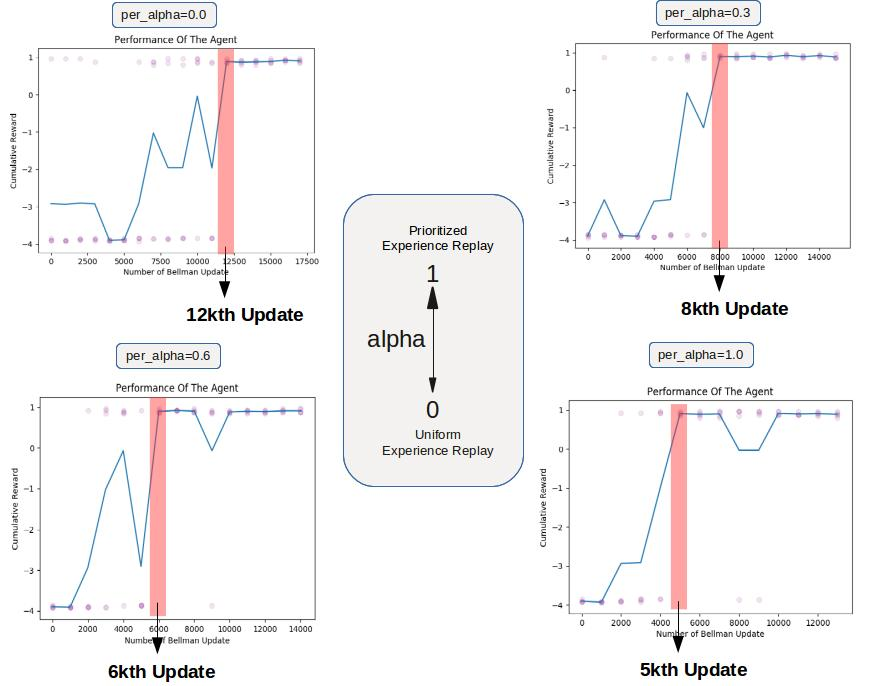
\includegraphics[width=0.7\textwidth]{prioritizeder3}
	\end{center}
	\caption{Simulations with different alpha parameters of prioritized experience replay.
		\label{fig:prioritizeder3}}
\end{figure}

\subsection{Comparison of Uniform vs Prioritized Experience Replays}
Figure \ref{fig:prioritizeder2} shows a comparison of different experience replay settings for same multi-agent grid world problem. It can be clearly seen that from 1st and 2nd simulations in the figure, Prioritized Experience Replay highly efficient when converging to optimum state. 

\begin{figure}[h]
	\begin{center}
		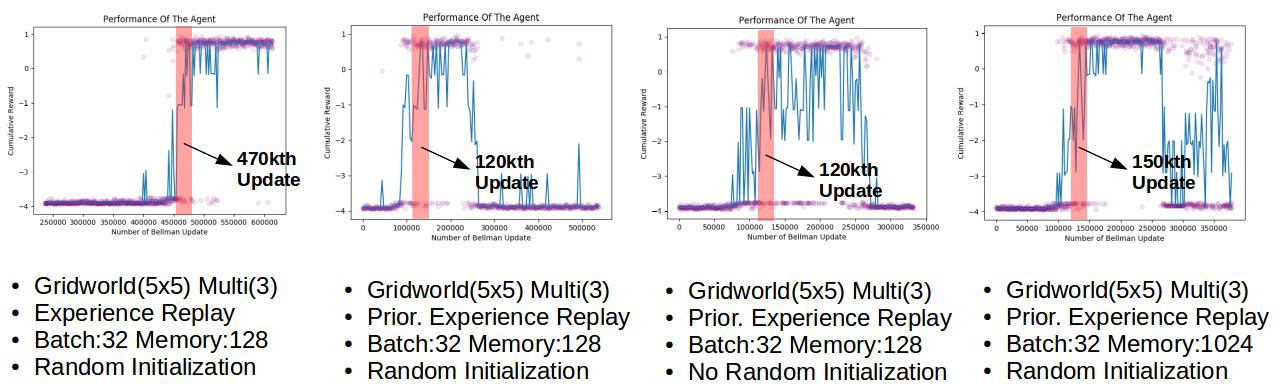
\includegraphics[width=1\textwidth]{prioritizeder2}
	\end{center}
	\caption{Comparison of Uniform vs Prioritized Experience Replays.
		\label{fig:prioritizeder2}}
\end{figure}

\section{STUDIES DURING THE LAST SIX MONTHS INCLUDED IN TIME PLAN BUT NOT CONDUCTED AND REASONS}
There is no study that is not conducted during the last six months. 

\section{CHANGES IN THE METHODOLOGY AND THEIR REASONS}
There is no change in the methodology.

\section{EXPLANATION OF THE STUDIES PLANNED FOR THE NEXT SIX MONTHS}
According to plan, in the next work package, multiagent planning algorithms will be developed using convolutional networks and tested on persistent surveillance environment. A convolutional network is also a kind of feedforward deep network, with convolutional layers, pooling layers. Convolutional neural networks (CNNs) are designed to process multiple data such as images, language, audio, and video \cite{li2017deep}. By using CNNs with reinforcement learning, the learning tasks can be generalized by processing images instead of problem-specific states. CNNs help agents to artificially learn from images. The deep convolutional networks are used as a function approximator for our quality and policy functions. The network can learn from just visual features from raw pixels and generate new strategies to get the maximum reward.

Besides deep convolutional networks, policy gradient approach is also utilized to improve the scalability of the multiagent system. Especially in multi-agent centralized setting, the joint action vector can be factorized into individual components for each agent \cite{gupta2017cooperative}. By the help of policy gradient method, the output of our network policy will just indicate each agent action distribution instead of joint action quality values as seen in Figure \ref{fig:convpolicygradient}. In a multi-agent system with discrete actions it significantly reduces the size of action space from $\| A^n \| $ to $n\|A\|$ where $A$ is action space for just a single agent and $n$ is the number of agents.

\begin{figure}[h]
	\begin{center}
		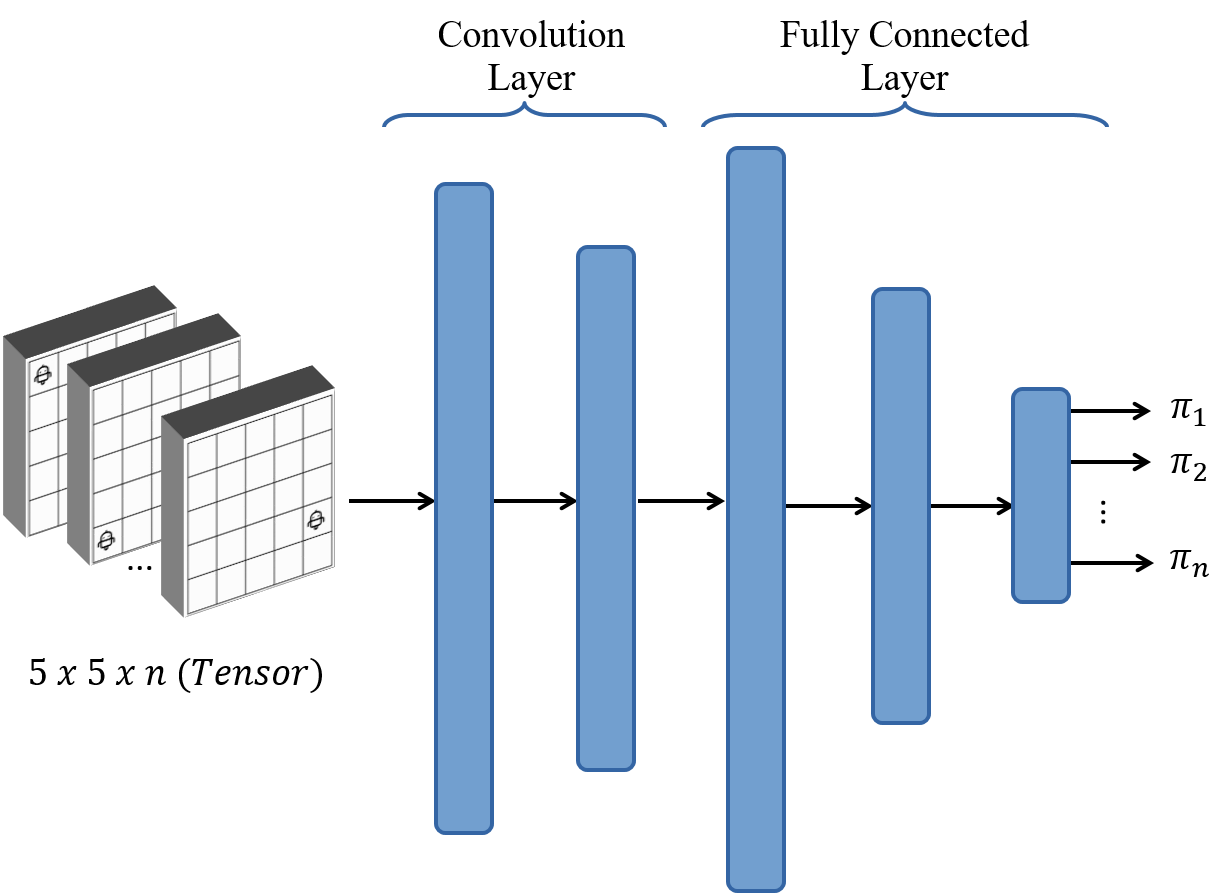
\includegraphics[width=0.6\textwidth]{convpolicygradient}
	\end{center}
	\caption{Convolutional networks and policy gradient are planned to be utilized in next six months for multiagent planning.
		\label{fig:convpolicygradient}}
\end{figure}

\section{PUBLICATIONS ABOUT THE THESIS SUBJECT BEING PREPARED AND/OR SUBMITTED}
According to time plan, the publications will be published prior to start of third phase which is Decentralized Multiagent Planning Phase.

\newpage
\bibliographystyle{ieeetr}
\bibliography{references}

\end{document}
